Although the synchronization protocol is one of the defining factors in simulation performance, model allocation has a significant impact on which protocol is ideal, and even whether or not parallelization would make sense.
Indeed, if the model is distributed in such a way that frequent communication is necessary between cores, parallelism is naturally reduced.
This thus brings us to the topic of model allocation.
Model allocation was one of the features also implemented by PythonPDEVS~\cite{PythonPDEVS2}.

The modeller can specify which kernel a model should be allocated to, should such manual intervention be required.
This is handled by the default model allocator.
If no preference is given a simple striping scheme is followed but this is not sufficient in most simulations to achieve a speedup in parallel.
By overriding the default allocator a modeller tunes the allocation scheme for a specific model, maximizing parallel speedup.
This interface can be used to employ graph algorithms for an automatic allocation scheme, for example avoiding cycles in the dependency graph.

\subsection{Performance Evaluation}
%TODO do basic performance evaluation of allocation
%TODO show model in statistics view
In order to evaluate the influence of model allocation, we define a new model, based on PHOLD~\cite{PHOLD}.
The model structure resembles a tree: an atomic model can have a set of children, with children being connected to each other as well.
Connections can be uni- or bidirectional.

Unlike the Queue model, the width of the hierarchy is still present in the topology of the atomic models after the direct connection stage.
The PHOLDTree model allows us to investigate parallel speedup in terms of model allocation, by modifying the depth and width (fanout) model parameters.

PHOLDTree can be used to model gossiping in social networks, hierarchical resource sharing or load balancing.
The lookahead of an atomic node is $\epsilon$, simulating uncertainty as will be often the case in real world models.
We demonstrate the importance of allocation, by comparing a breadth-first versus a depth-first scheme.

\begin{figure}
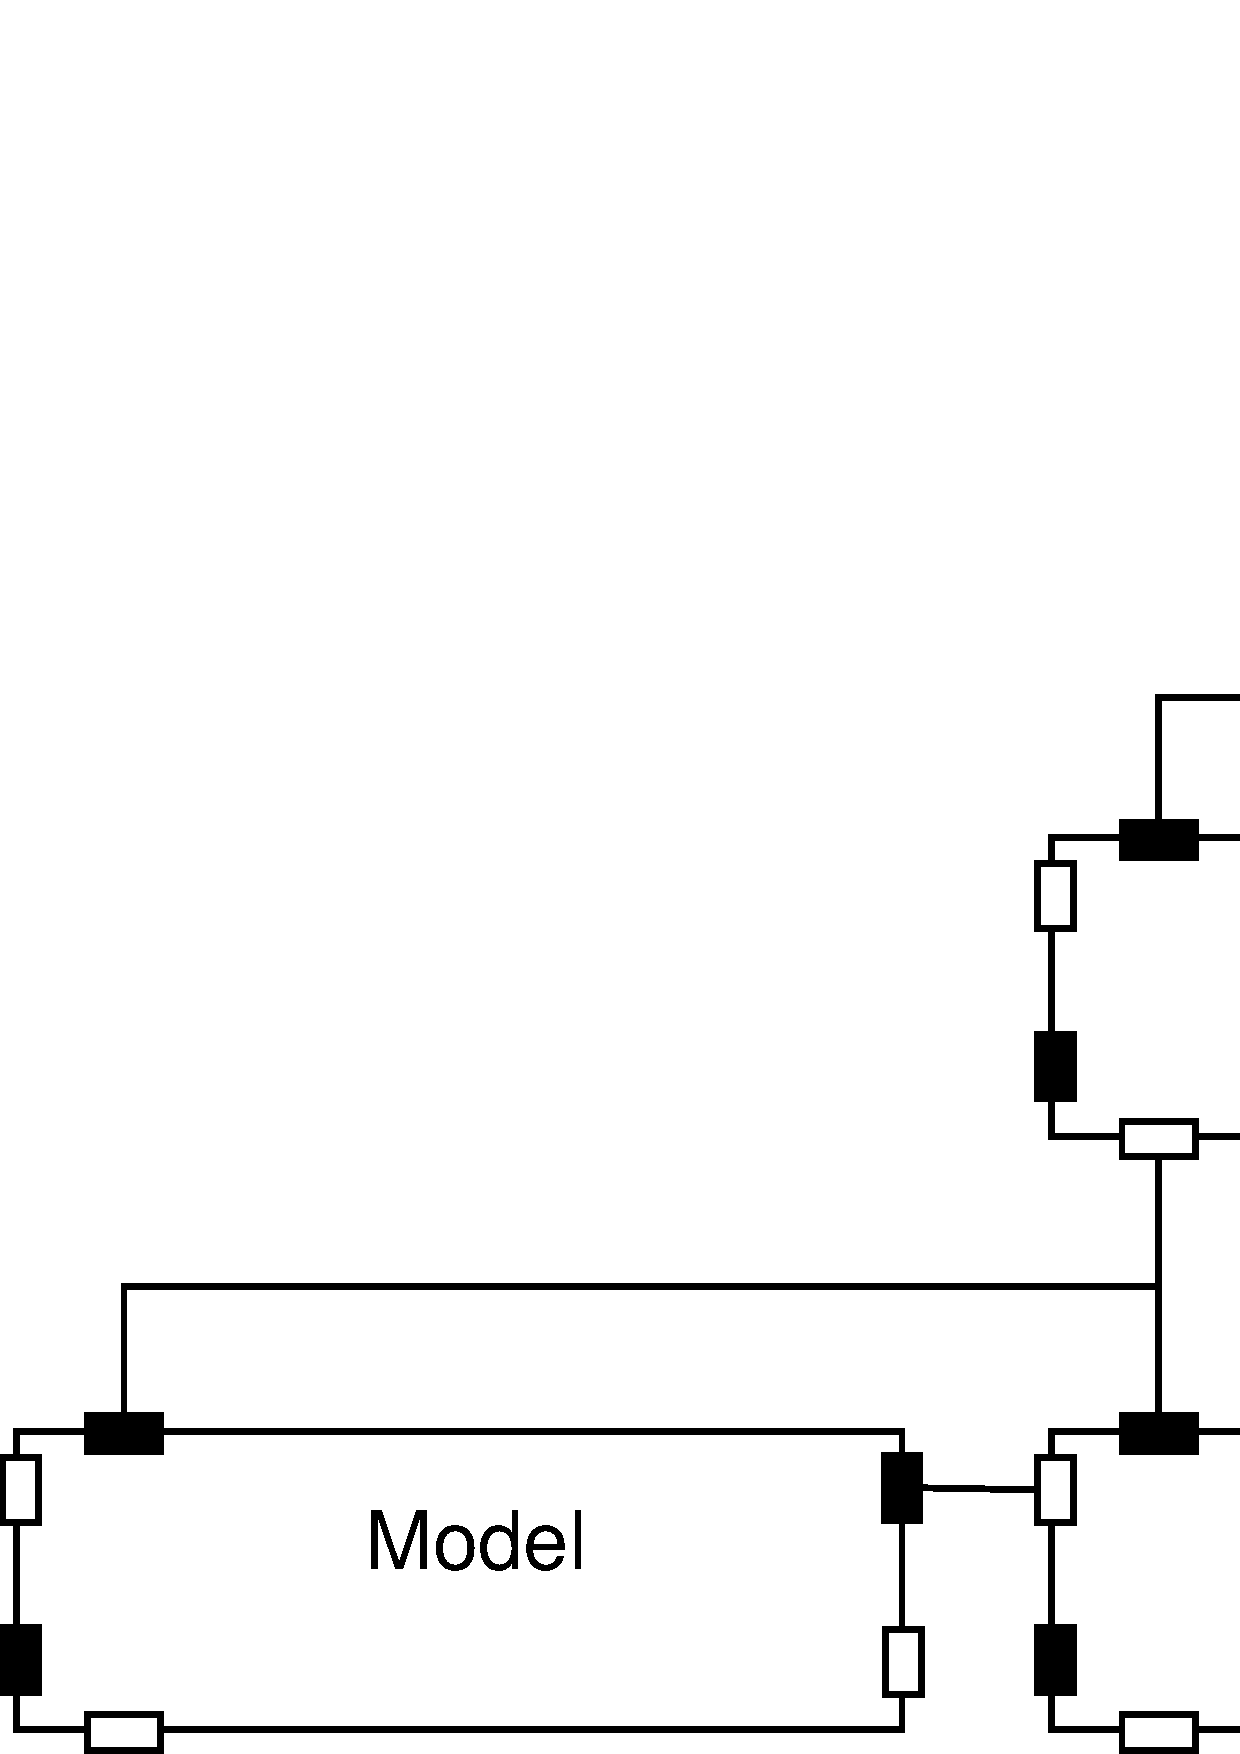
\includegraphics[width=\modelfraction\columnwidth]{fig/pholdtree.pdf}
%TODO depth 1 but 3 levels deep?
\caption{PHOLDTree model for depth 1 and width 2.}
\label{fig:PHOLDTree_model}
\end{figure}

PHoldtree, like Queue, is a highly hierarchical model but one where the flattened structure cannot be partitioned into a chain as in Queue.
This topology is interesting since it highlights the effects of allocation which we have shown already in PHold and Interconnect to be of vital importance.
This model allows us to investigate in depth the effects of non-cyclic allocation strategies and measure parallel speedup.

Since adevs does not use the directconnect algorithm, we expect some performance penalty between dxex and adevs.
The event frequency in PHoldTree can be configured to highlight dxex's performance disadvantage here as shown in the Interconnect benchmark.

\paragraph*{Event frequency}
Similarly when the probability on a priority event (p) increases the amount of event generated will increase and thus the runtime.
In Figure~\ref{fig:PHoldtree_seq_p_benchmark} we observe that p has a near linear impact on performance, with the shape of the curve due to rounding errors.
The advantage adevs has in simulations where event frequency is high has been demonstrated by the interconnect benchmark.

\paragraph*{Hierarchy}
To establish a baseline for the parallel simulation benchmarks we measure how the PHoldTree benchmark performs sequentially when we vary each of the model's parameters.
When we increase the depth and fanout of the model, we expect to see an increase in runtime.
In Figure~\ref{fig:PHoldtree_seq_dn_benchmark} the n parameter (fanout) determines the performance penalty adevs suffers compared to dxex.

If we compare the instances d=2, n=2 with d=2, n=4, which show a clear difference in performance between adevs and dxex, we conclude from the profiling callgraphs that the increase in width per subtree (n) leads to higher overhead for adevs.
Dxex in contrast uses the directconnect algorithm and has no such overhead.
An increase in n will rapidly increase the number of connections \ref{eq:pholdtreelinkcount} (and thus the routing problem adevs faces), whereas d will increase modelcount \ref{eq:pholdtreemodelcount} faster but have a lesser impact on connections.
Both kernels scale linear in increasing number of atomic models.

\begin{figure}
    \center
    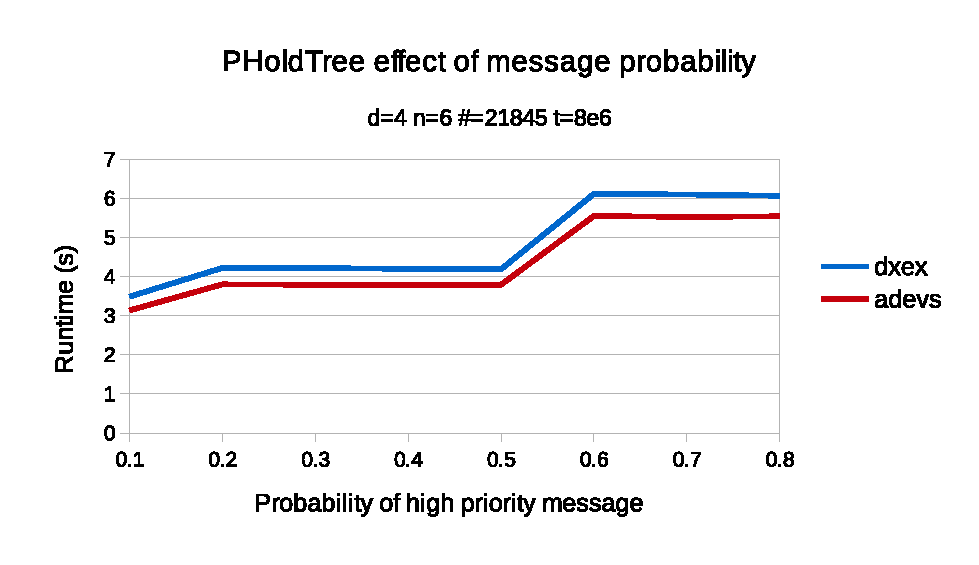
\includegraphics[width=\plotfraction\columnwidth]{fig/pholdtree_sequential_p.eps}
    \caption{PHoldTree for increasing probability of priority message.}
    \label{fig:PHoldtree_seq_p_benchmark}
\end{figure}
% Img for p increasing
\begin{figure}
    \center
    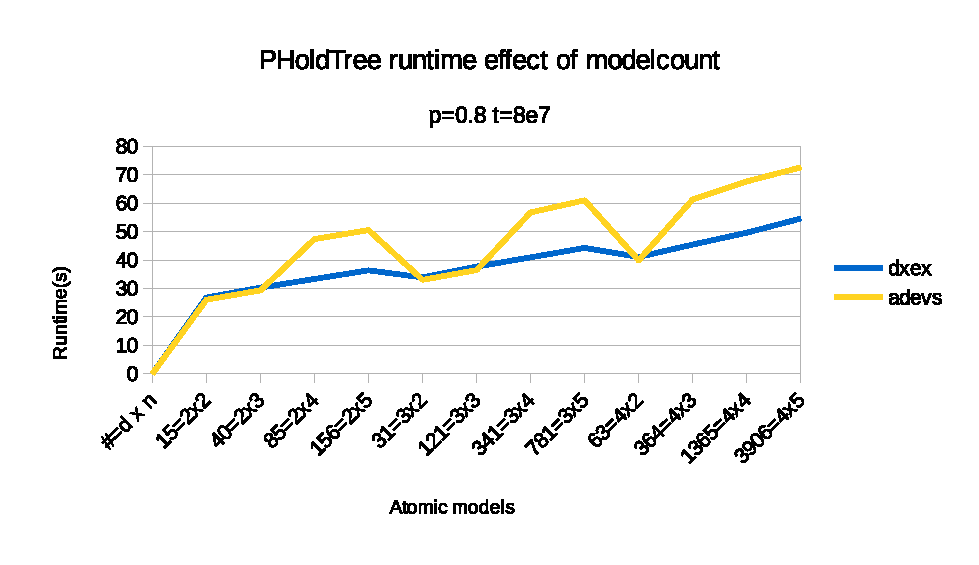
\includegraphics[width=\plotfraction\columnwidth]{fig/pholdtree_sequential_dn.eps}
    \caption{PHoldTree : Effect of hierarchy.}
    \label{fig:PHoldtree_seq_dn_benchmark}
\end{figure}

We further verify that our contribution fulfills our projected use case: a single model that can be tweaked to favor either conservative or optimistic synchronization. We will demonstrate that allocation is critical to achieve a parallel speedup and that the configuration of the model will give either conservative or optimistic an advantage.
\paragraph*{Allocation}\label{PholdTreeallocation}
The PholdTree benchmark can be configured to use 2 allocation schemes: breadth first and depth first.
The breadth first allocation scheme will result in kernels that will form a dependency chain with multiple branches, much like in the Queue model.
Such a linear dependency chain can result in a parallel speedup as we demonstrated with the Queue model, but this is not always true as we will demonstrate in this section.
A single kernel that has an unbalanced number of atomic models or unequal computation load in transition functions will slow down the remainder of the chain. This effect is also apparent if the thread a kernel runs on is not fairly scheduled. In conservative this will lead to excessive polling of the other kernels' eot values, in optimistic this will lead to a cascade of reverts since dependent kernels will simulate ahead of the slower kernel. In Figures \ref{fig:pholdtree_visualize_parBFS} and \ref{fig:pholdtree_visualize_parDFS} the simulation trace is visualized for both allocation schemes highlighting the remarks made in this paragraph.
%
%\begin{figure}
%   \center
%   
%   \includegraphics[width=\modelfraction\columnwidth]{fig/pholdtreeBFS.eps}
%   \caption{PholdTree model breadth first allocation with 3 kernels.}
%   \label{fig:PholdTree_model_bfs}
%   
%   \includegraphics[width=\modelfraction\columnwidth]{fig/pholdtreeDFS.eps}
%   \caption{PholdTree model depth first allocation with 3 kernels.}
%   \label{fig:PholdTree_model_dfs}
%\end{figure}

\paragraph*{Strong Scaling}\label{pholdtreestrongscale}
In Figure \ref{fig:PholdTree_plot_alloc_high} we see that the difference in performance for all 4 kernel configurations compared to that shown in Figure \ref{fig:PholdTree_plot_alloc_low} is a constant factor. The probability of the priority message has no extra impact on performance other than that shown in sequential performance.

The probability of a high priority event in this model does not affect the performance difference between conservative and optimistic. The key parameter quickly becomes the load of a kernel in models. Our conservative implementation in an uncertain simulation is very sensitive to a high load in models, whereas optimistic has no such limitation.

The difference between depth first and breadth first allocated kernels is striking, the first results in sublinear speedup for both synchronization protocols. %reword 
The breadth first allocation scheme will lead to a very high number of inter-kernel connections, which is detrimental for any parallel synchronization algorithm. An event exchanged between kernels cannot be securely deallocated without a GVT algorithm and all the complexity this entails. Even a fast asynchronous GVT algorithm will require some form of inter kernel synchronization and span a timeframe during which allocated memory cannot be reused, forcing new allocations.
Similar to the Queue benchmark the breadth first allocation scheme leads to a topology for the kernels resembling a chain but with more branches in the chain. In Queue there is only a single model on the edge of a kernel exchanging messages to a single other model in a neighbouring kernel, this is not the case in the PholdTree under breadth first allocation. This explains the difference in speedup between Queue and PholdTree despite the similarity in kernel topology.\\
Depth first allocation still has a higher inter kernel connection count, but not on the same order as breadth first allocated PholdTree. Depth first allocation will converge to a star topology which in this benchmark leads to a significant speedup.\\
The performance drop observed for 2 kernels for all allocation schemes and synchronization protocols is in part due to the higher link count between kernels. With more kernels these connections will be spread across more kernels and result in a relative lower performance penalty. \\
Conservative synchronization suffers a further penalty in this benchmark when there are only a few kernels. The PholdTree model has a lookahead of $\epsilon$ leading the kernel to query each allocated atomic model for a lookahead value on each simulation round. As the atomic models are spread over more kernels this effect is reduced leading to an increase in performance. With 4 kernels conservative surpasses optimistic in speedup. This is clear evidence that conservative synchronization is a good candidate for parallel simulation even in simulations with uncertainty.
\begin{figure}
    \center

    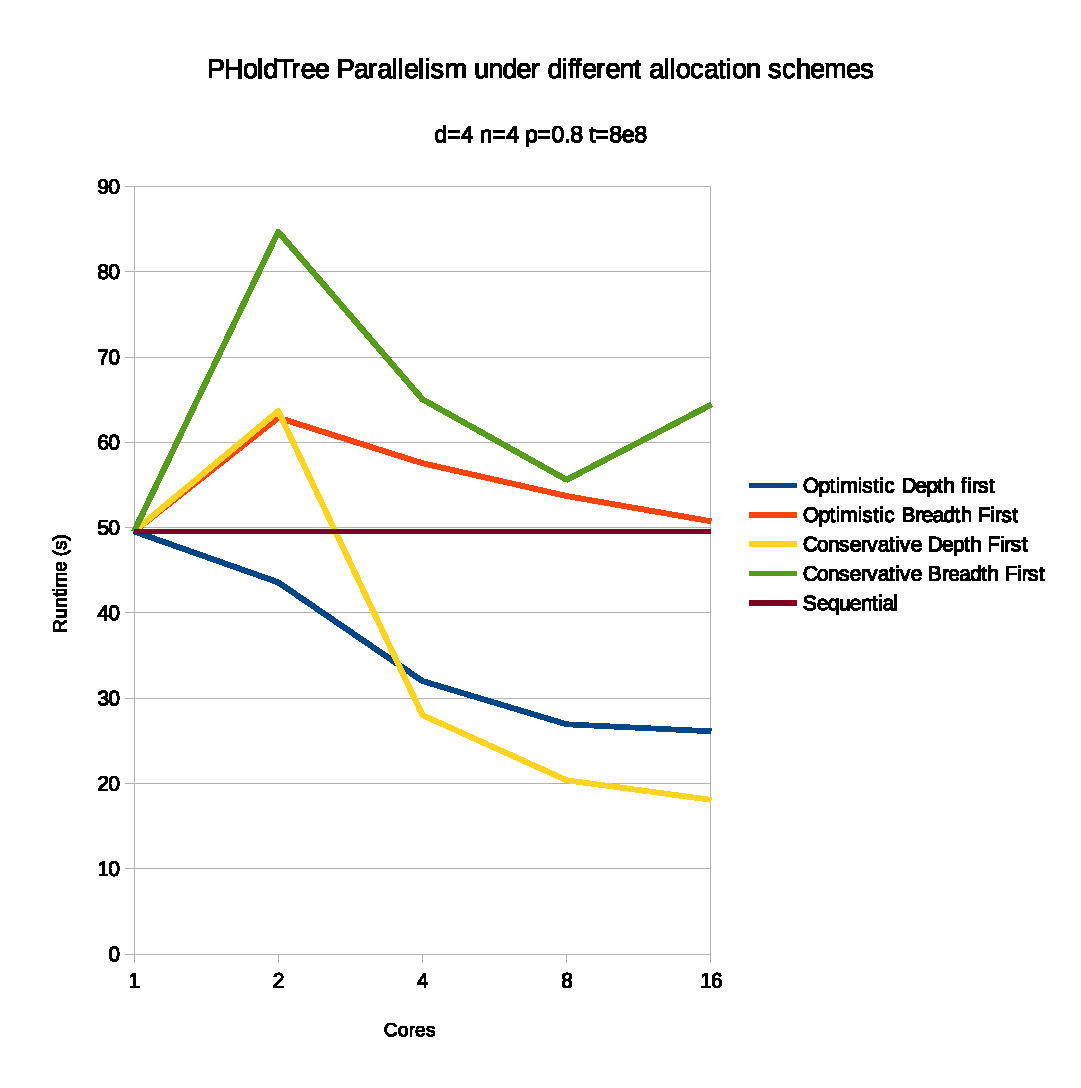
\includegraphics[width=\modelfraction\columnwidth]{fig/pholdtreealloclowp.eps}
    \caption{PholdTree model performance under different allocation schemes with low message probability}
    \label{fig:PholdTree_plot_alloc_low}

    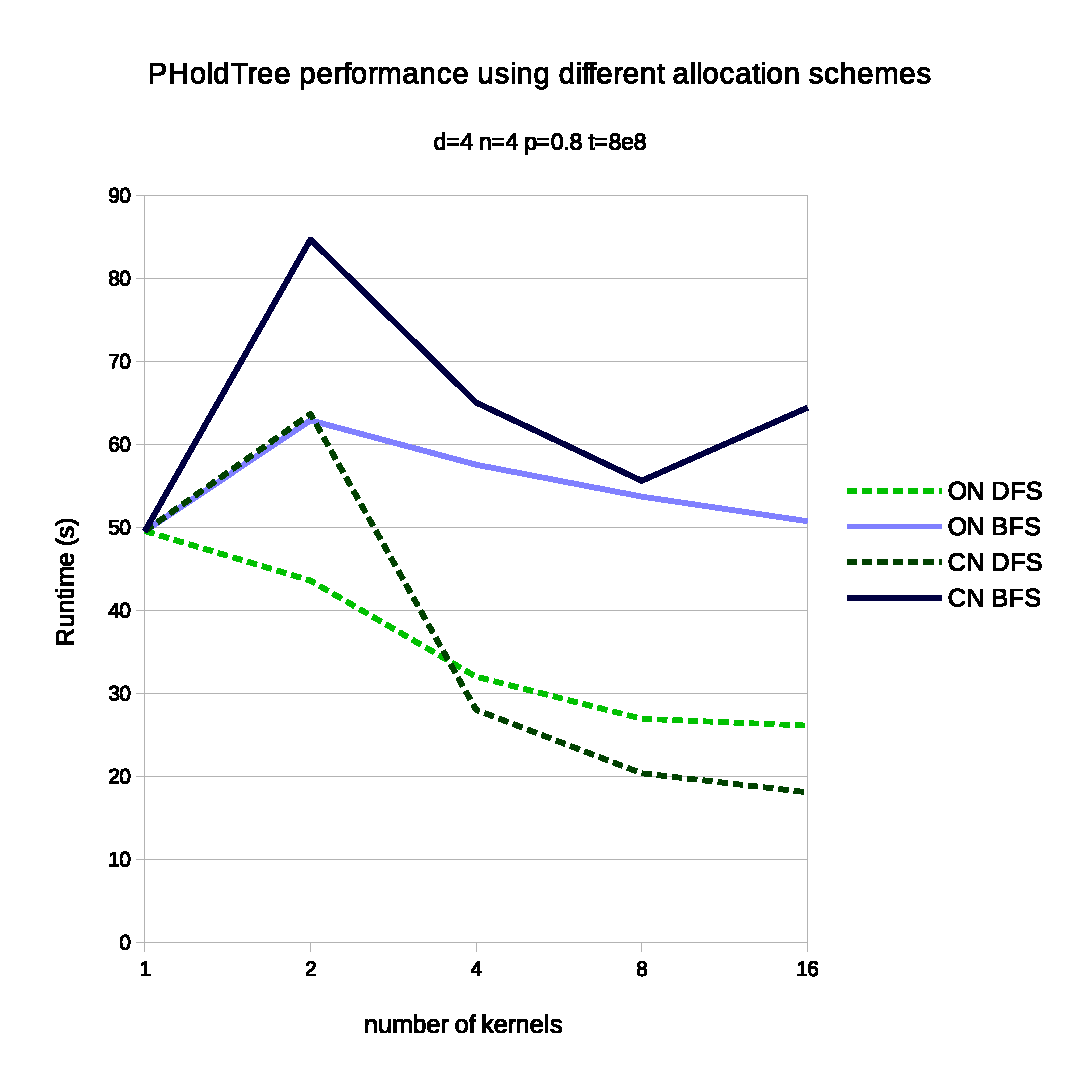
\includegraphics[width=\modelfraction\columnwidth]{fig/pholdtreeallochighp.eps}
    \caption{PholdTree model performance under different allocation schemes with high message probability}
    \label{fig:PholdTree_plot_alloc_high}
\end{figure}

\paragraph*{Weak Scaling}
%Intro
In this paragraph we investigate dxex's parallel performance when the the number of atomic models distributed over a fixed number of kernels varies. From \ref{eq:pholdtreemodelcount} we know that increasing d will lead to a very rapid increase in models. We want to observe what happens in a closer to linear increase in model count per kernel by varying n.

% Explain why adevs is not plotted (its x100 slower)
Adevs' conservative implementation cannot handle the uncertainty (lack of non $\epsilon$ lookahead) here and is omitted from the comparison. Its parallel performance is two orders of magnitude slower than the sequential implementation. Upon investigation we conclude that this slowdown is caused by not implementing the \{begin/end\}lookahead() functions, which when not overridden in a model trigger an exception on each invocation.
This exception handling completely stalls the kernel. We do not implement this function in our PholdTree variant for adevs since this would force us to implement state saving in the model code and not use the provided state saving functionality in the kernel, as is done in dxex or PythonPDEVS's optimistic.
In dxex state saving is never required for a conservative simulation, this is handled transparently for the user who need not implement this behaviour.
By using the state saving technique inside the model code we feel we would no longer compare identical models across different synchronization algorithms, although we do not doubt adevs' increased performance when these functions are overridden.

% Optimistic
In Figure \ref{fig:PholdTree_plot_weaknopt} we observe that dxex's optimistic kernels are slightly sensitive to the number of atomic models allocated to them. In the worst case with 2 kernels there is no real speedup observable, as soon as the number of kernels increases we see a converging speedup trend, that except for 32 kernels is almost constant despite the increase in n. Note that only depth first allocated kernels are measured here, breadth first as we can see in \ref{fig:PholdTree_plot_alloc_high} has no speedup advantage. The probability parameter is kept at 0.1 for the same reason, it only induces a linear increase in load.

% Conservative
Conservative has a more nuanced speedup behaviour in this benchmark. We have detailed how a conservative kernel in dxex scales linear in the number of atomic models (if lookahead is $\epsilon$), this effect is more clearly visible here. \\
It is clear that as the fanout (n) of the model increases the kernel performance degrades rapidly. The intersection of the performance graph of each configuration is shifted to the right, the actual 1-speedup point increases as the kernelcount increases. For a d=4, n=5 configuration with 4 kernels each kernel has a load of ~1300 atomic models when it crosses the 1-speedup line. \\
An 8 kernel configuration with d=4 n=6 can sustain a load of ~2700 atomic models before it reaches that point. From the results we see that the 32-kernel configuration is not yet slowing down with the current parameters. \\
The modelcount is only a part of the explanation of this effect, as the kernelcount increases the amount of inter kernel messages will be split into more distinct sets which can be handled with more concurrency in dxex's architecture.
That this effect is not always true can be observed from the d=4 n=3 32-kernel datapoint. Note that in this configuration 341 atomic models are distributed over 32 kernels, a relative low model load can more easily highlight synchronization overhead, even if allocation is optimal.\\
As with optimistic we do not include breadth first allocated benchmarks in this speedup plot since none of those achieve a speedup higher than 1.
\\
If we combine both to determine which synchronization protocol is more optimal we see in Figure \ref{fig:PholdTree_plot_weakall} that for these configurations conservative with 8 kernels is an ideal configuration up until n=5, where the modelcount starts to degrade performance. Optimistic with the same kernelcount is almost insensitive to the increase in modelcount and is therefore a more robust choice. Note how optimistic and conservative with 32 kernels at this point still have a reasonable speedup which is surprising given the synchronization overhead in such a large set of kernels.
\begin{figure}
    \center

    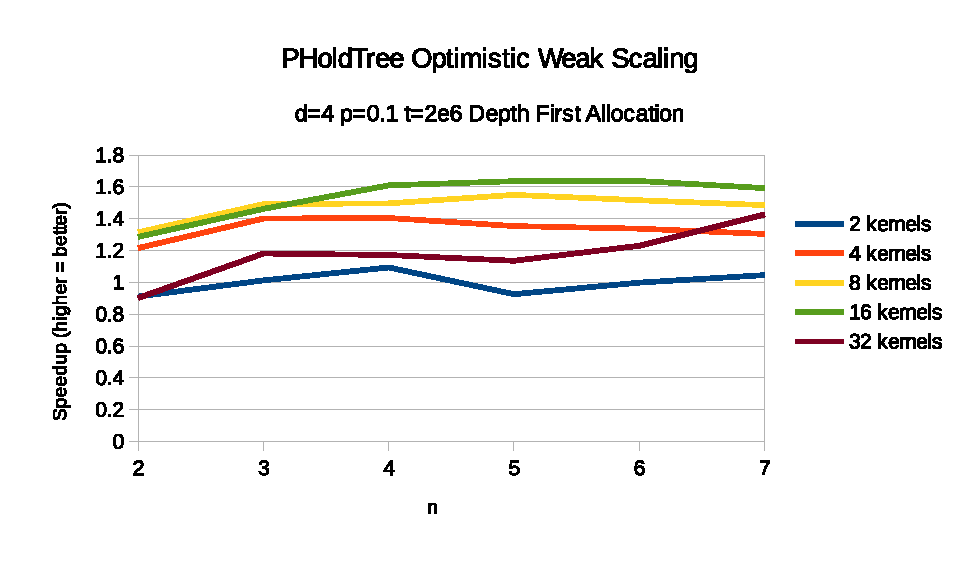
\includegraphics[width=\modelfraction\columnwidth]{fig/pholdtreeweakscalingnopt.eps}
    \caption{PholdTree model weak scaling under varying fanout and optimistic synchronization}
    \label{fig:PholdTree_plot_weaknopt}

    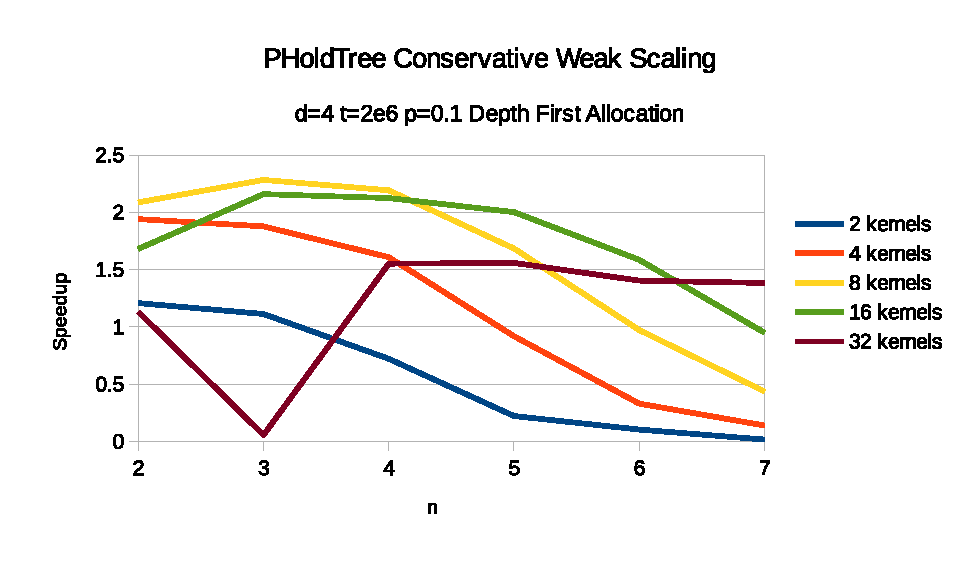
\includegraphics[width=\modelfraction\columnwidth]{fig/pholdtreeweakscalingncon.eps}
    \caption{PholdTree model weak scaling under varying fanout and conservative synchronization}
    \label{fig:PholdTree_plot_weakncon}

    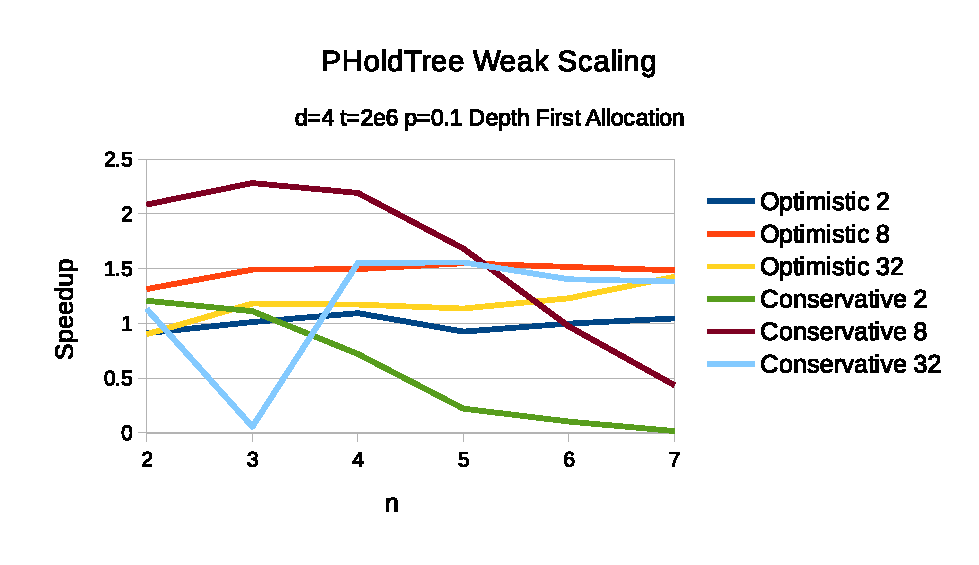
\includegraphics[width=\modelfraction\columnwidth]{fig/pholdtreeweakscalingall.eps}
    \caption{PholdTree model weak scaling under varying fanout and different synchronization algorithms}
    \label{fig:PholdTree_plot_weakall}
\end{figure}

\subsection{Linking Back}
%TODO link back to initial performance evaluation

\begin{figure}
    \center
    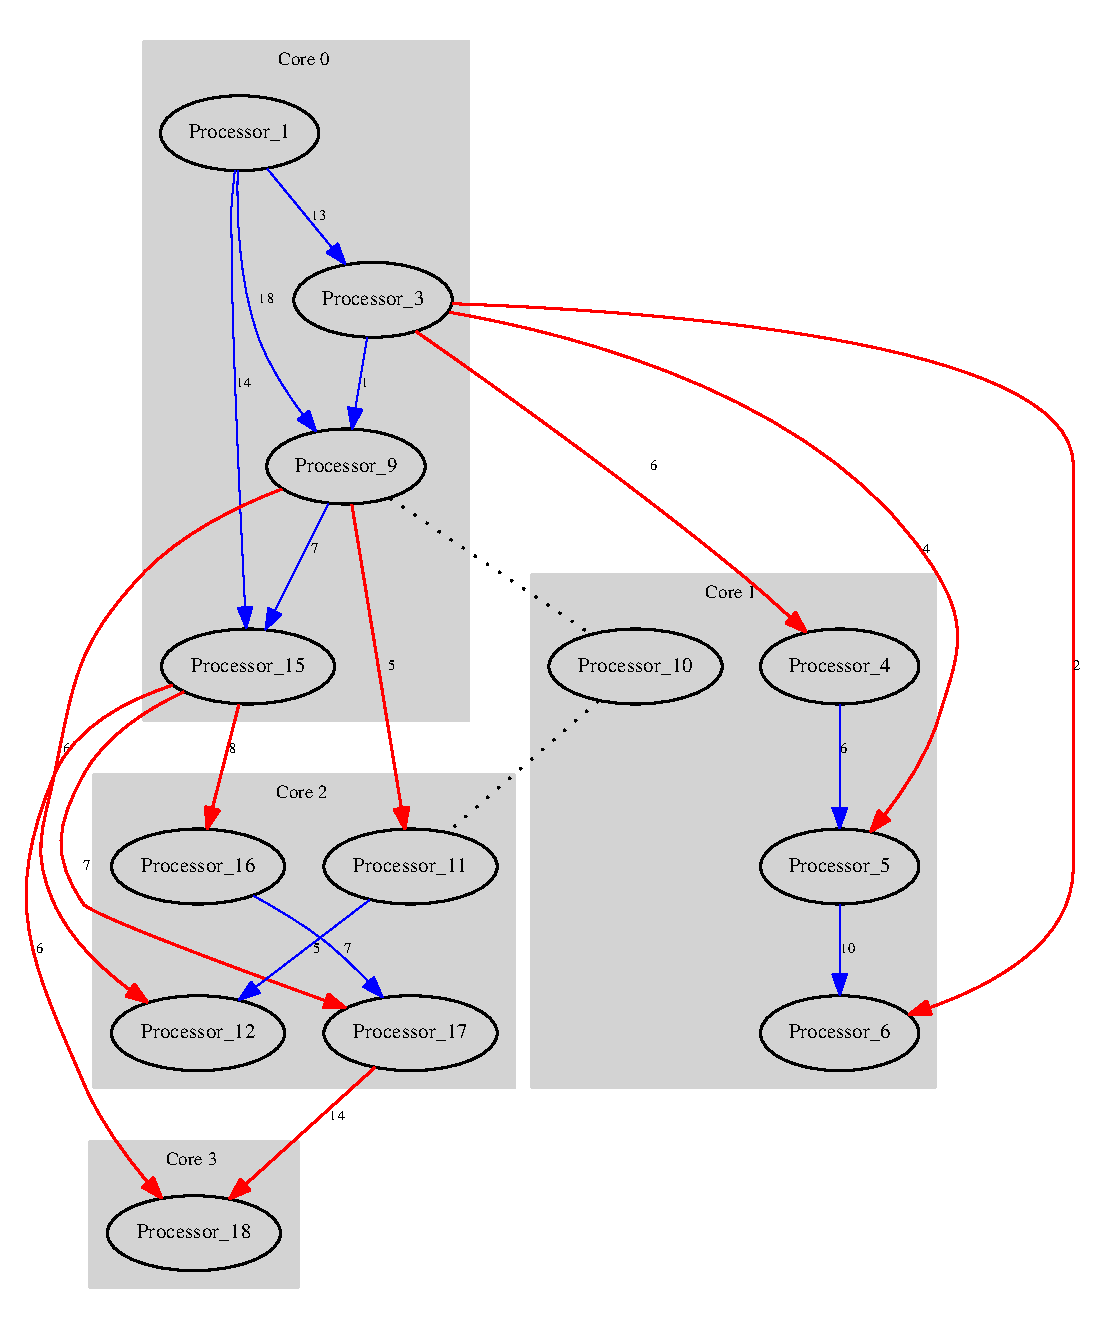
\includegraphics[width=\plotfraction\columnwidth,  height=6cm, keepaspectratio]{fig/pholdtreed1n3t5000c4BFS.eps}
    \caption{Visualization of PholdTree (d=1,n=3,t=5000) parallel simulation with breadth first allocation and 4 kernels.}
    \label{fig:pholdtree_visualize_parBFS}
\end{figure}
\begin{figure}
    \center
    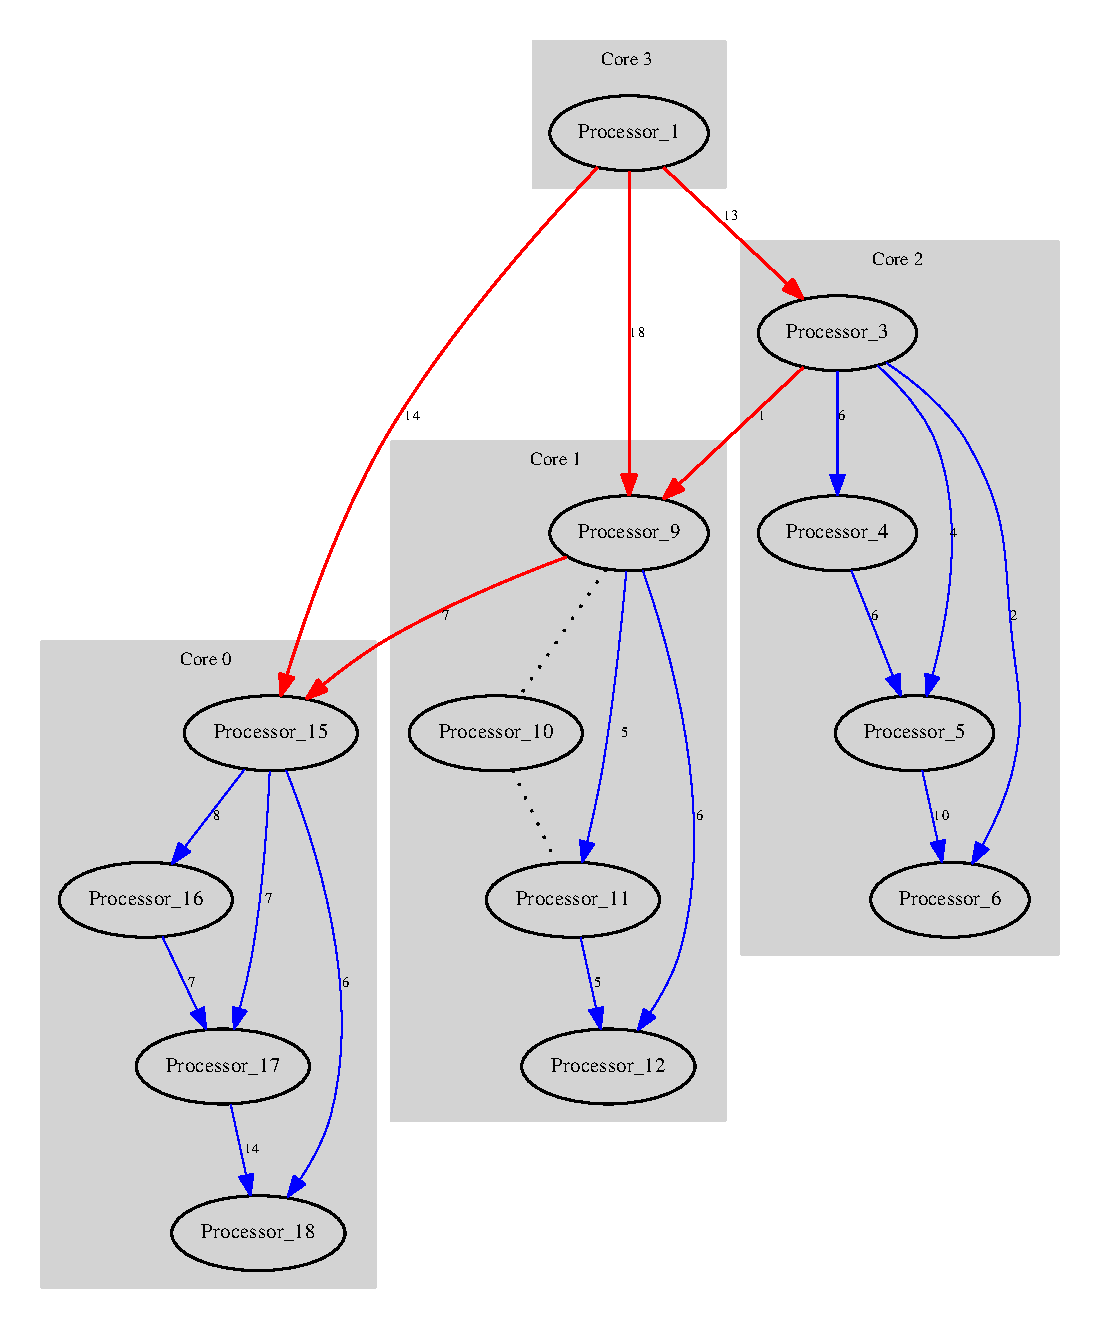
\includegraphics[width=\plotfraction\columnwidth,  height=6cm, keepaspectratio]{fig/pholdtreed1n3t5000c4DFS.eps}
    \caption{Visualization of PholdTree (d=1,n=3,t=5000) parallel simulation with depth first allocation and 4 kernels.}
    \label{fig:pholdtree_visualize_parDFS}
\end{figure}
